\subsubsection{Zone Construction}\label{alg:zon_construction}
The graph coloring algorithm used by the MAPC server to determine occupied zones is described in detail in the scenario description (\texttt{scenario.pdf}) included in the 2014 MAPC download package and will not be explained again here. To position themselves in an optimally-scoring way, agents could use the same algorithm on their side to calculate the agent placement that will lead to the highest total sum of zone scores in each step. However, the number of ways to place $n$ agents on $k$ nodes is $C \left (n+r-1,r-1\right )= \frac{\left(n+r-1 \right )!}{n!\left(r-1 \right )!}$, a number that increases rapidly with $n$ and $k$. In particular, there are $C \left (28+600-1,600-1 \right ) = 3.7463887025070038e+48$ ways to place 28 agents on 600 nodes - far too many to calculate in real-time.

\iffalse % comments out the following
Due to the way the server-side colouring algorithm works, placing $N$ agents on the map so that they establish the highest possible zone value per step is anything but straight-forward. Even for $n = 1$, a single agent placed on an articulation point in the graph can establish a high-value zone if there are no enemy agents in either subgraph that it splits the map into. \autoref{fig:articulation_points} shows an example.
\begin{figure}
  \centering
  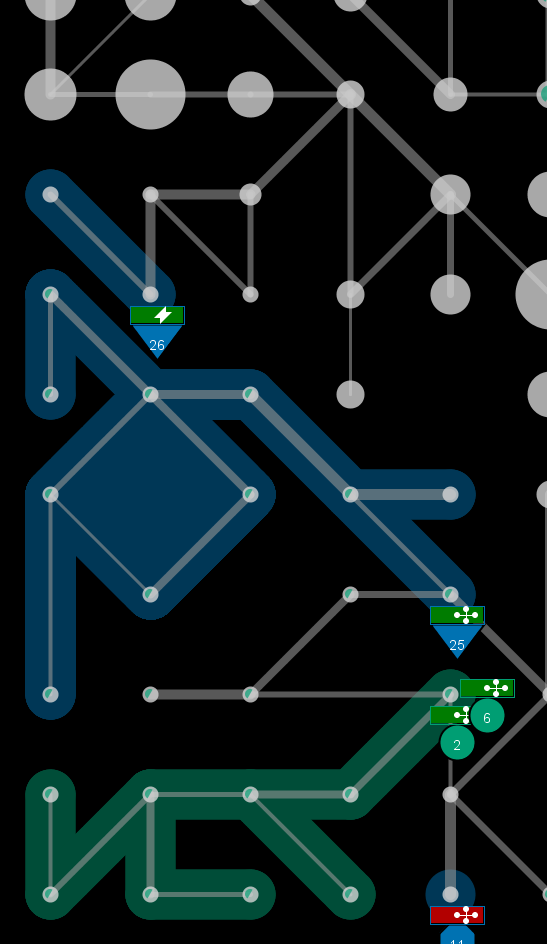
\includegraphics[width=\gri\textwidth]{articulation_points}
  \caption{The control loop for the agent deliberation process in the BOID architecture. Taken from \citeauthor{broersen2002goal}~\cite{broersen2002goal}.}
  \label{fig:control}
\end{figure}
In some way, we try to find local maxima to build small zones with as few agents as possible. How do we find zones? How do we find out how many agents we need? Explain that extending zones describes how the score resulting from an active zone can be increased by using idle agents. How do we determine what additional spots for zone extensions exist?
Present our colouring algorithm and the concept of a centre node.
\fi